\section{Apresentação}

\begin{frame} % Capa
    \titlepage
\end{frame}

\begin{frame}{Apresentação}
    \begin{itemize}
        \item Professor {\fontfamily{augie}\selectfont Rodrigo de Farias Gomes}
        \item Telefone (somente mensagens): (92) 9 9405-1724
        \item E-mail: shpnft@gmail.com

    \end{itemize}

    \centering

    \vspace{2cm}
    \begin{tabular}{cccccc}
        R & G & O & M & E & S \\ \\
        \(\color{red} \left.\phantom{{\scriptstyle +1}\frac{1}{2}}\right\downarrow {\scriptstyle +1}~~\) &
        \(\color{red} \left.\phantom{{\scriptstyle +1}\frac{1}{2}}\right\downarrow {\scriptstyle +1}~~\) &
        \(\color{red} \left.\phantom{{\scriptstyle +1}\frac{1}{2}}\right\downarrow {\scriptstyle +1}~~\) &
        \(\color{red} \left.\phantom{{\scriptstyle +1}\frac{1}{2}}\right\downarrow {\scriptstyle +1}~~\) &
        \(\color{red} \left.\phantom{{\scriptstyle +1}\frac{1}{2}}\right\downarrow {\scriptstyle +1}~~\) &
        \(\color{red} \left.\phantom{{\scriptstyle +1}\frac{1}{2}}\right\downarrow {\scriptstyle +1}~~\) \\ \\
        S & H & P & N & F & T
    \end{tabular}
\end{frame}

\begin{frame}{Calendário}
    \centering
    \small{
        \begin{tabular}{cP{2cm}P{2cm}P{2cm}P{2cm}P{2cm}}
            \rowcolor{black!10} & Segunda & Terça & Quarta & Quinta & Sexta \\
            01 & \dma{0} & \dma{1} & \dma{2} & \dma{3} & \dma{4} \\
            02 & \dma{7} & \dma{8} & \dma{9} & \dma{10} & \dma{11} \\
            03 & \dma{14} & \dma{15} & \dma{16} & \dma{17} & \dma{18} \\
            04 & \dma{21} & \dma{22} & \dma{23} & \dma{24} & \dma{25} \\
            05 & \dma{28} & \dma{29} & \dma{30} & \dma{31} & \dma{32} \\
            06 & \dma{35} & \dma{36} & \dma{37} & \dma{38} & \dma{39} \\
            07 & \dma{42} & \dma{43} & \dma{44} & \dma{45} & \dma{46} \\
            08 & \dma{49} & \dma{50} & \dma{51} & \dma{52} & \dma{53} \\
            09 & \dma{56} & \dma{57} & \dma{58} & \dma{59} & \dma{60} \\
            10 & \dma{63} & \dma{64} & \dma{65} & \dma{66} & \dma{67} \\
            11 & \dma{70} & \dma{71} & \dma{72} & \dma{73} & \dma{74} \\
            12 & \dma{77} & \dma{78} & \dma{79} & \dma{80} & \dma{81} \\
            13 & \dma{84} & \dma{85} & \dma{86} & \dma{87} & \dma{88} \\
            14 & \dma{91} & \dma{92} & \dma{93} & \dma{94} & \dma{95} \\
            15 & \dma{98} & \dma{99} & \dma{100} & \dma{101} & \dma{102} \\
            % 16 & \dma{103} & \dma{104} & \dma{105} & \dma{106} & \dma{107} \\
            % 17 & \dma{108} & \dma{109} & \dma{110} & \dma{111} & \dma{112} \\
        \end{tabular}
    }
\end{frame}

\begin{frame}{Meus horários em 20/03/2023...}
    \small{
        \begin{center}
            \begin{tabular}{ccccc}
                \rowcolor{black!10} Segunda & Terça & Quarta & Quinta & Sexta \\ \hline
                \rowcolor{red!25} &&&& \\ \hline
                \rowcolor{red!25} Métodos Num... & Trigonometria & Métodos Num... & Trigonometria & \\ \hline
                \rowcolor{green!25} & & Termodinâmica & & Termodinâmica \\ \hline
                \rowcolor{green!25} & Óptica e Eletro... & & Óptica e Eletro... & \\ \hline
                \rowcolor{blue!25} &&&& \\ \hline
                \rowcolor{blue!25} &&&& \\ \hline
            \end{tabular}
        \end{center}

        \vspace{1cm}
        Legenda:
        \begin{itemize}
            \item[\textcolor{red!25}{\rule{1em}{1em}}] Manhã (8:00 -- 10:00 e 10:00 -- 12:00)
            \item[\textcolor{green!25}{\rule{1em}{1em}}] Tarde (14:00 -- 16:00 e 16:00 -- 18:00)
            \item[\textcolor{blue!25}{\rule{1em}{1em}}] Noite (18:00 -- 20:00 e 20:00 -- 22:00)
        \end{itemize}
    }
\end{frame}

\begin{frame}[label=ementa]{Ementa de \Disciplina}
    \begin{itemize}
        \item Conceitos fundamentais
        \item Equação de estado
        \item Primeira Lei da Termodinâmica
        \item Algumas consequências da Primeira Lei
        \item Entropia e Segunda Lei da Termodinâmica
        \item Primeira e Segunda Leis combinadas
        \item Potenciais termodinâmicos
        \item Aplicações da termodinâmica a sistemas simples
        \item Forças intermoleculares
        \item Física Estatística
        \item Aplicações da Física Estatística a gases e outros sistemas
    \end{itemize}
\end{frame}

\begin{frame}{Avaliação}
    \begin{itemize}
        \item A avaliação será na forma de 3 notas: \(N_1\), \(N_2\) e \(N_3\)
        \item A média dos exercícios escolares (\(MEE\)) será dada por
            \[
                MEE=\frac{N_1+N_2+N_3}{3}
            \]
        \item Se \(MEE \geq 8,0\), então a média final (\(MF\)) será igual à \(MEE\)
        \item Se \(MEE < 8,0\), então
            \[
                MF=\frac{2\times MEE+PF}{3}
            \]
            onde PF é a nota da \textbf{prova final}
        \item Se \(MF \geq 5,0\) e a frequência em sala for maior que 75\%, o aluno está aprovado
        \item Haverá 30 aulas de \SI{2}{horas}, de forma que \textbf{o número máximo de faltas é 8}
    \end{itemize}
\end{frame}

\begin{frame}{Livro}
    \centering
    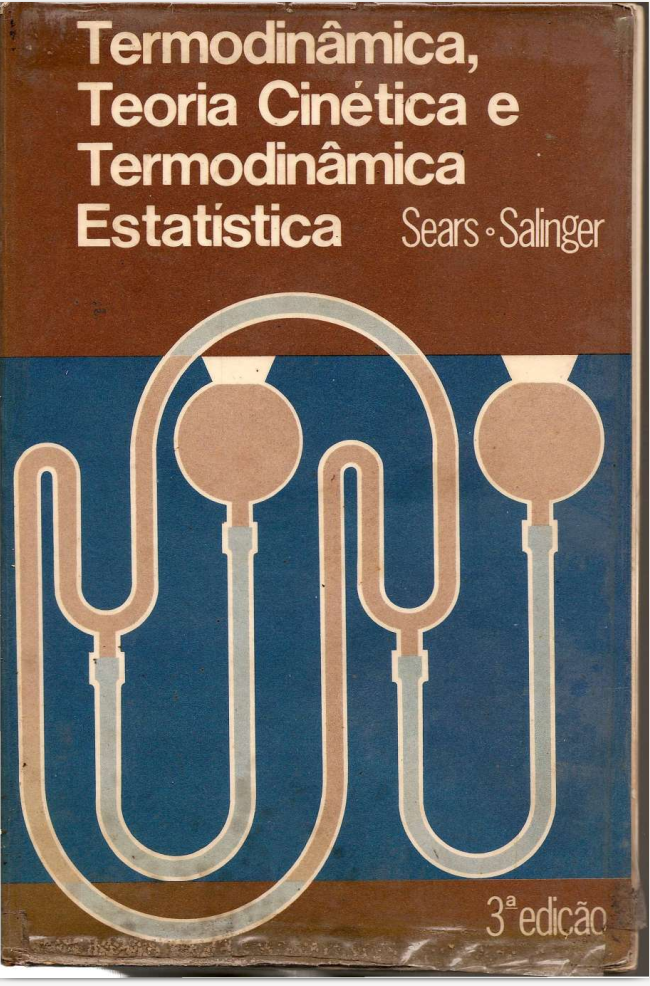
\includegraphics[height=0.8\textheight]{images/Captura de tela de 2023-03-27 07-48-28.png}
\end{frame}

\begin{frame}
    \centering
    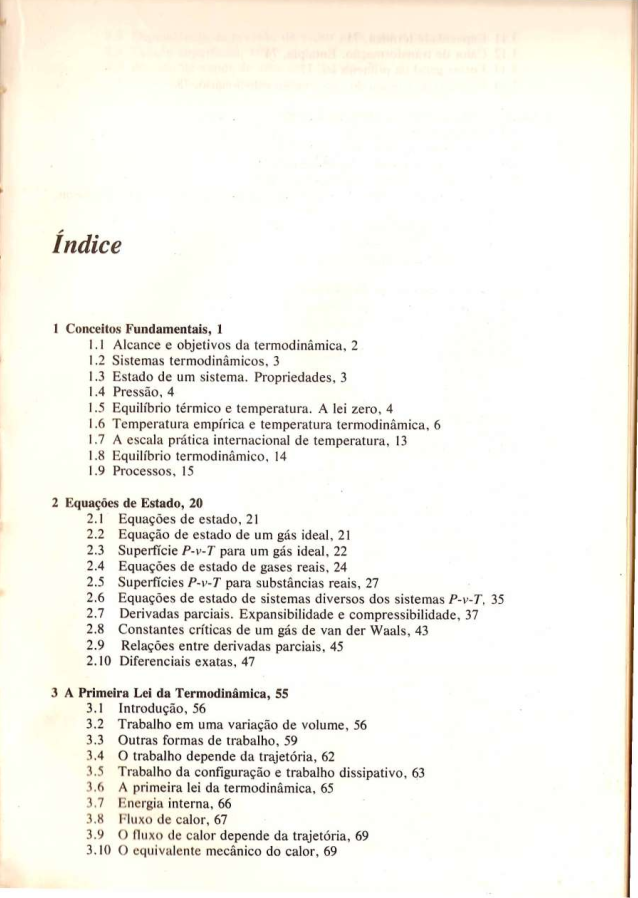
\includegraphics[width=0.32\textwidth]{images/Captura de tela de 2023-03-27 07-48-56.png}
    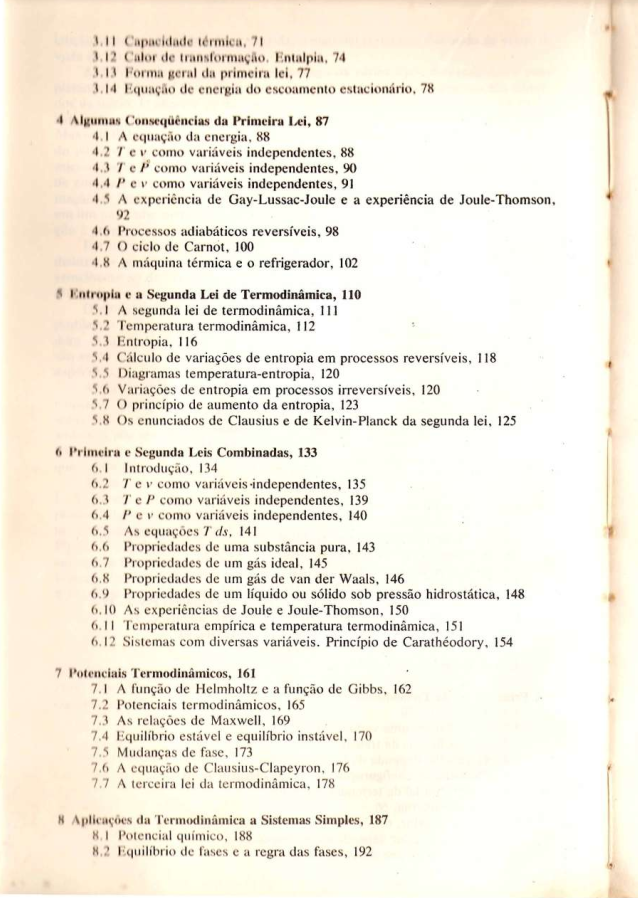
\includegraphics[width=0.32\textwidth]{images/Captura de tela de 2023-03-27 07-49-06.png}
    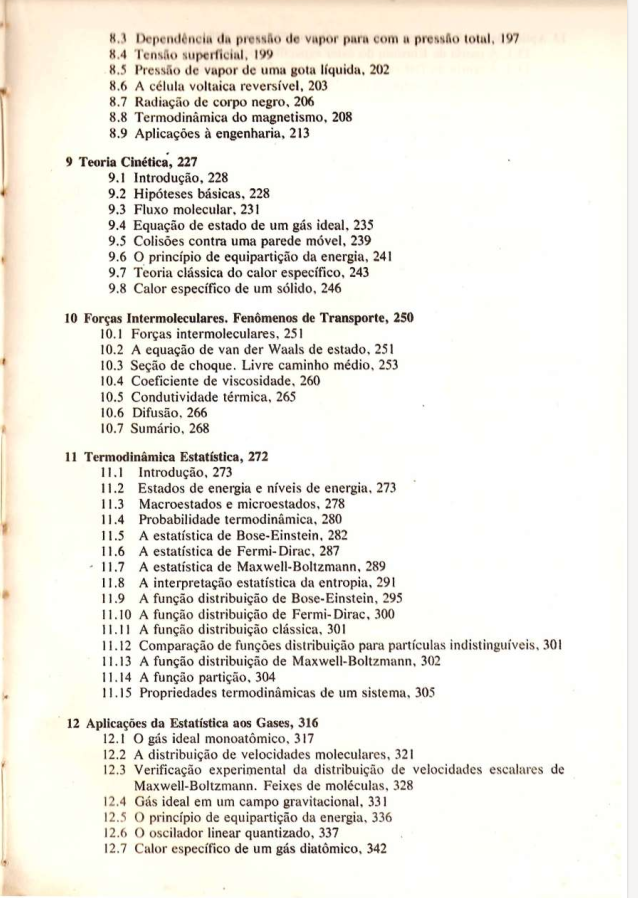
\includegraphics[width=0.32\textwidth]{images/Captura de tela de 2023-03-27 07-49-18.png}
\end{frame}

\againframe<2>{ementa}

\begin{frame}[c]{Termodinâmica}
    \begin{minipage}{\textwidth}
        \color{blue}
        Se as teorias físicas fossem pessoas, a Termodinâmica seria a bruxa da
        aldeia. Ao longo de três séculos, ela sorriu silenciosamente enquanto
        outras teorias surgiam e desapareciam, sobrevivendo a grandes
        revoluções na Física, como o advento da relatividade geral e da
        mecânica quântica. As outras teorias a acham um tanto estranha, de
        alguma forma de natureza diferente do restante, mas todos vêm a ela em
        busca de conselhos e ninguém ousa contradizê-la. Einstein, por exemplo,
        chamou-a de “a única teoria física de conteúdo universal, que estou
        convencido de que dentro da estrutura de aplicabilidade de seus
        conceitos básicos nunca será derrubada”
    \end{minipage}

    \vspace{1cm}
    John Goold \textit{et al} 2016 J. Phys. A: Math. Theor. 49 143001 \\
    https://doi.org/10.1088/1751-8113/49/14/143001
\end{frame}

\begin{frame}[c]{Leis da Termodinâmica, versão poltrona do vovô}
    \begin{itemize}
        \item Lei zero: Se você tocar em alguma coisa, você entra no jogo
        \item Lei um: A vida é um jogo
        \item Lei dois: Você não pode vencer
        \item Lei três: Você não pode nem empatar
    \end{itemize}

    \vspace{1cm}
    Escrito por Thomas Tabb Mayo IV
\end{frame}

\begin{frame}[c]{Mecânica Estatística}
    \begin{minipage}{\textwidth}
        \color{blue}
        Ludwig Boltzmann, who spent much of his life studying statistical
        mechanics, died in 1906, by his own hand. Paul Ehrenfest, carrying on the
        work, died similarly in 1933. Now it is our turn to study statistical
        mechanics.
    \end{minipage}

    \vspace{1cm}
    Texto de David L. Goodstein no livro \textit{States of Matter} (1975)
\end{frame}

\begin{frame}{Então...}
    \begin{itemize}
        \item A Termodinâmica é uma ciência experimental, baseada em um pequeno
            número de princípios, que são generalizações feitas a partir da
            experiência
        \item \textcolor{red}{Ela trabalha apenas com as propriedades \textit{macroscópicas} da
            matéria}
        \item Dos princípios da termodinâmica podemos obter relações gerais
            entre grandezas físicas e como essas dependem da temperatura.
        \item Os princípios da termodinâmica nos dizem quais as relações entre as 
            grandezas físicas que devem ser experimentalmente determinadas para que 
            \textit{todas} as propriedades do sistema sejam \textit{completamente} determinadas
    \end{itemize}
\end{frame}
